\documentclass[12pt]{article}
\usepackage{amsmath, amssymb, amsthm}
\usepackage{geometry, enumitem, mdframed}
\usepackage{tikz, pgfplots}
\usepackage{array}
\geometry{margin=1in}

\newtheorem{definition}{Definition}
\newtheorem{theorem}{Theorem}
\newtheorem{example}{Example}
\newmdenv[linecolor=blue,linewidth=2pt]{keypoint}
\newmdenv[linecolor=red,linewidth=2pt]{warning}
\newmdenv[linecolor=green,linewidth=2pt]{insight}

\title{ODE Lesson 8: Parameter-Dependent Existence Problems}
\author{ODE 1 - Prof. Adi Ditkowski}
\date{}

\begin{document}
\maketitle

\section{Introduction to Parametric ODEs}

\begin{definition}[Parametric ODE]
A \textbf{parametric ODE} has the form:
$y' = f(x, y; \mu)$
where $\mu$ is a parameter (or vector of parameters) that affects the equation's behavior.
\end{definition}

\begin{keypoint}
\textbf{Key Questions for Parametric Problems:}
\begin{enumerate}
    \item For which $\mu$ does a solution exist?
    \item For which $\mu$ is it unique?
    \item How does the solution behavior change with $\mu$?
    \item Where are the bifurcation points?
\end{enumerate}
\end{keypoint}

\section{Parameter Location Analysis}

\subsection{Where Parameters Appear}

\begin{table}[h]
\centering
\begin{tabular}{|l|l|l|}
\hline
\textbf{Location} & \textbf{Example} & \textbf{Main Concern} \\
\hline
Coefficients & $y' = \mu y$ & Usually safe \\
Denominators & $y' = \frac{y}{x-\mu}$ & Singularities \\
Exponents & $y' = |y|^\mu$ & Lipschitz condition \\
Initial conditions & $y(0) = \mu$ & Starting point issues \\
Domain bounds & $y' = \sqrt{\mu - y^2}$ & Real-valued constraints \\
\hline
\end{tabular}
\end{table}

\section{Critical Parameter Values}

\begin{definition}[Critical Parameter]
A \textbf{critical parameter value} $\mu_c$ is where:
\begin{itemize}
    \item The number of equilibria changes
    \item Stability of equilibria changes
    \item Existence/uniqueness properties change
    \item Solution behavior undergoes qualitative change
\end{itemize}
\end{definition}

\section{Standard Examples}

\subsection{Example 1: Linear with Parameter}

\begin{example}[Exponential Growth/Decay]
$y' = \mu y, \quad y(0) = 1$

Analysis:
\begin{itemize}
    \item Solution exists for all $\mu$: $y = e^{\mu x}$
    \item Behavior changes at $\mu = 0$:
    \begin{itemize}
        \item $\mu < 0$: Exponential decay to 0
        \item $\mu = 0$: Constant solution
        \item $\mu > 0$: Exponential growth to $\infty$
    \end{itemize}
\end{itemize}
\end{example}

\begin{center}
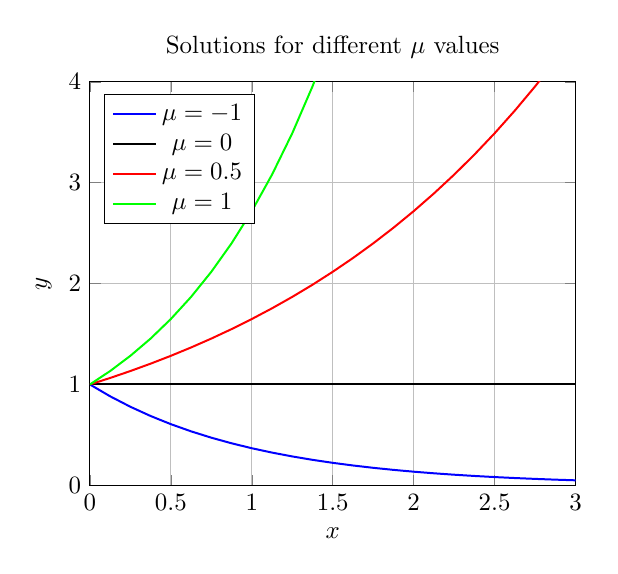
\begin{tikzpicture}[scale=0.9]
\begin{axis}[
    xlabel={$x$},
    ylabel={$y$},
    grid=major,
    xmin=0, xmax=3,
    ymin=0, ymax=4,
    legend pos=north west,
    title={Solutions for different $\mu$ values}
]
\addplot[blue, thick, domain=0:3] {exp(-x)};
\addlegendentry{$\mu = -1$}
\addplot[black, thick, domain=0:3] {1};
\addlegendentry{$\mu = 0$}
\addplot[red, thick, domain=0:3] {exp(0.5*x)};
\addlegendentry{$\mu = 0.5$}
\addplot[green, thick, domain=0:3] {exp(x)};
\addlegendentry{$\mu = 1$}
\end{axis}
\end{tikzpicture}
\end{center}

\subsection{Example 2: Parameter in Denominator}

\begin{example}[Moving Singularity]
$y' = \frac{y}{x - \mu}, \quad y(0) = 1$

Analysis by parameter:
\begin{itemize}
    \item $\mu < 0$: Solution exists for all $x \geq 0$
    \item $\mu = 0$: No solution through $(0,1)$ (singularity at initial point)
    \item $\mu > 0$: Solution exists for $x \in [0, \mu)$, blows up at $x = \mu$
\end{itemize}

General solution (when it exists): $y = \frac{C}{x - \mu}$
\end{example}

\subsection{Example 3: Parameter Affects Lipschitz}

\begin{example}[Uniqueness Switch]
$y' = \mu|y|^{1/2}, \quad y(0) = 0$

Analysis:
\begin{itemize}
    \item $\mu = 0$: Unique solution $y \equiv 0$
    \item $\mu \neq 0$: Not Lipschitz at $y = 0$, infinitely many solutions
\end{itemize}

Solution family for $\mu \neq 0$:
$y(x) = \begin{cases}
    0 & \text{if } |x| \leq c \\
    \frac{\mu^2}{4}(x-c)^2 & \text{if } x > c \geq 0
\end{cases}$
\end{example}

\section{Bifurcation Analysis}

\subsection{Types of Bifurcations}

\begin{definition}[Bifurcation]
A \textbf{bifurcation} occurs at parameter value $\mu_c$ where the qualitative structure of solutions changes.
\end{definition}

\begin{table}[h]
\centering
\begin{tabular}{|l|l|l|}
\hline
\textbf{Type} & \textbf{Equation Form} & \textbf{Behavior} \\
\hline
Saddle-node & $y' = \mu - y^2$ & Equilibria appear/disappear \\
Transcritical & $y' = \mu y - y^2$ & Equilibria exchange stability \\
Pitchfork & $y' = \mu y - y^3$ & Symmetry breaking \\
Hopf & System of ODEs & Periodic orbits appear \\
\hline
\end{tabular}
\end{table}

\subsection{Pitchfork Bifurcation Example}

\begin{example}[Pitchfork]
$y' = \mu y - y^3$

Equilibria: $y = 0$ and $y = \pm\sqrt{\mu}$ (if $\mu > 0$)

\begin{itemize}
    \item $\mu < 0$: Only $y = 0$ (stable)
    \item $\mu = 0$: Only $y = 0$ (critically stable)
    \item $\mu > 0$: Three equilibria:
    \begin{itemize}
        \item $y = 0$ (unstable)
        \item $y = \pm\sqrt{\mu}$ (stable)
    \end{itemize}
\end{itemize}
\end{example}

\begin{center}
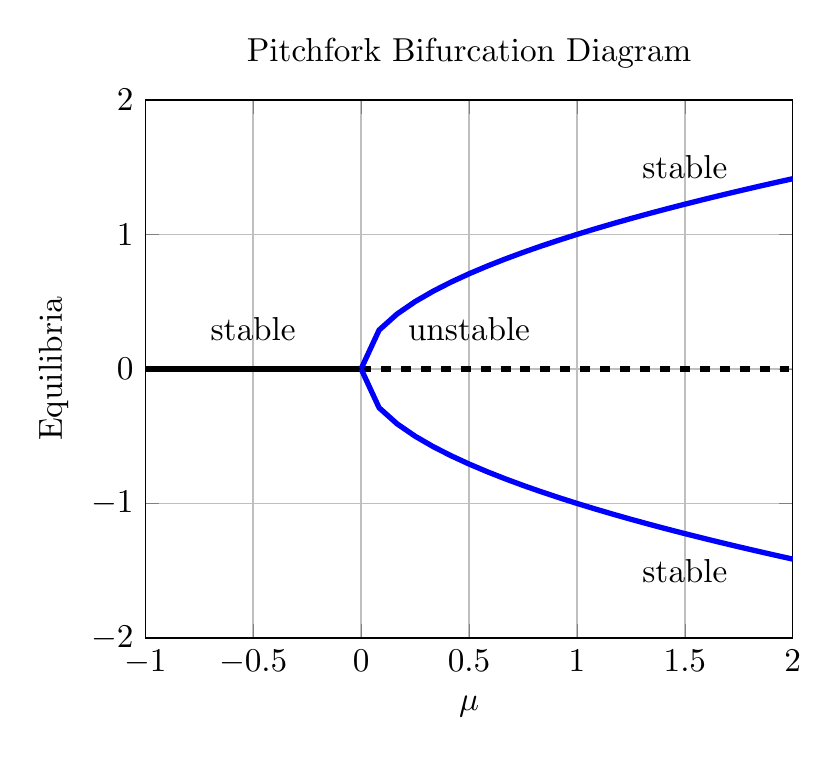
\begin{tikzpicture}[scale=1.2]
\begin{axis}[
    xlabel={$\mu$},
    ylabel={Equilibria},
    grid=major,
    xmin=-1, xmax=2,
    ymin=-2, ymax=2,
    title={Pitchfork Bifurcation Diagram}
]
% Stable branch y=0 for mu<0
\addplot[black, ultra thick, domain=-1:0] {0};
% Unstable branch y=0 for mu>0
\addplot[black, dashed, ultra thick, domain=0:2] {0};
% Upper stable branch
\addplot[blue, ultra thick, domain=0:2] {sqrt(x)};
% Lower stable branch
\addplot[blue, ultra thick, domain=0:2] {-sqrt(x)};
\node at (axis cs:-0.5,0.3) {stable};
\node at (axis cs:0.5,0.3) {unstable};
\node at (axis cs:1.5,1.5) {stable};
\node at (axis cs:1.5,-1.5) {stable};
\end{axis}
\end{tikzpicture}
\end{center}

\section{Riccati Equation with Parameter}

\begin{example}[Parametric Riccati]
$y' = y^2 - \mu$

Analysis:
\begin{itemize}
    \item $\mu < 0$: No real equilibria, all solutions blow up
    \item $\mu = 0$: One equilibrium at $y = 0$ (semi-stable)
    \item $\mu > 0$: Two equilibria at $y = \pm\sqrt{\mu}$
\end{itemize}

Blow-up analysis:
\begin{itemize}
    \item If $|y_0| > \sqrt{\mu}$ (when $\mu > 0$): Solution blows up
    \item If $|y_0| < \sqrt{\mu}$: Solution remains bounded
    \item If $|y_0| = \sqrt{\mu}$: Solution approaches equilibrium
\end{itemize}
\end{example}

\section{Global Existence Criteria}

\begin{insight}
\textbf{For global existence, check:}
\begin{enumerate}
    \item No finite-time blow-up (solutions remain bounded)
    \item No singularities in the domain
    \item Lipschitz condition holds globally
\end{enumerate}
\end{insight}

\begin{example}[Global Existence Analysis]
$y' = y^2 + \mu y + 1$

Discriminant: $\Delta = \mu^2 - 4$

\begin{itemize}
    \item $|\mu| < 2$: No real equilibria, all solutions blow up
    \item $|\mu| = 2$: One equilibrium (double root)
    \item $|\mu| > 2$: Two equilibria, bounded solutions possible
\end{itemize}

For global existence: Need $|\mu| \geq 2$ and appropriate initial conditions.
\end{example}

\section{Continuous Dependence on Parameters}

\begin{theorem}[Continuous Dependence]
If $f$ and $\frac{\partial f}{\partial y}$ are continuous in $(x, y, \mu)$, then the solution $y(x, \mu)$ is continuous in $\mu$.
\end{theorem}

\begin{warning}
\textbf{Continuous $\neq$ Smooth!}
Small parameter changes can cause:
\begin{itemize}
    \item Bifurcations (structure changes)
    \item Blow-up time shifts
    \item Stability switches
    \item Period changes (for oscillatory solutions)
\end{itemize}
\end{warning}

\section{Singular Perturbations}

\begin{definition}[Singular Perturbation]
When a small parameter $\epsilon$ multiplies the highest derivative:
$\epsilon y'' + f(y', y, x) = 0$
As $\epsilon \to 0$, the order of the equation changes!
\end{definition}

\begin{example}[Fast-Slow System]
$\epsilon y' = -y + \mu$

\begin{itemize}
    \item For $\epsilon > 0$: First-order ODE with solution $y = \mu + (y_0 - \mu)e^{-x/\epsilon}$
    \item As $\epsilon \to 0^+$: Rapid transition to $y = \mu$
    \item At $\epsilon = 0$: Algebraic equation $y = \mu$
\end{itemize}

Time scale: $\tau = x/\epsilon$ shows fast dynamics.
\end{example}

\section{Parameter Identification}

\begin{mdframed}[backgroundcolor=yellow!10]
\textbf{Exam Question Type:} "Find all $\mu$ such that..."
\begin{enumerate}
    \item The solution exists globally
    \item All solutions are periodic
    \item The equilibrium at origin is stable
    \item The solution through $(0,1)$ remains bounded
\end{enumerate}
\end{mdframed}

\section{Systematic Analysis Strategy}

\begin{keypoint}
\textbf{Parameter Analysis Algorithm:}
\begin{enumerate}
    \item Identify where $\mu$ appears (coefficient, denominator, etc.)
    \item Find critical values (singularities, Lipschitz failure, etc.)
    \item Analyze each parameter regime separately
    \item Determine equilibria and their stability
    \item Check for bifurcations
    \item Sketch bifurcation diagram
    \item Consider limiting cases ($\mu \to 0, \pm\infty$)
\end{enumerate}
\end{keypoint}

\section{Memory Device}

\begin{center}
\textbf{PARAMETER Analysis:}\\
\textbf{P}osition (where is $\mu$?)\\
\textbf{A}nomalies (singularities)\\
\textbf{R}egimes (different cases)\\
\textbf{A}nalysis (each case)\\
\textbf{M}onotonicity (how solution changes)\\
\textbf{E}quilibria\\
\textbf{T}ransitions (bifurcations)\\
\textbf{E}xistence (global vs local)\\
\textbf{R}ate of change
\end{center}

\end{document}